\documentclass[quiz,addpoints,noanswers]{exam}

\usepackage[quiz]{../biology11}
\usepackage{chemformula}

\title{Quiz: Cell cycle}
\date{\today}
\author{\mobeardInstructorShort}

\begin{document}
\maketitle
%\begin{abstract}
%Today's quiz is a salute to Q1/Q2. This quiz should only take about \SI{5}{\minute}. Answers will be made available on Google Drive \SI{15}{\minute} after the quiz start time. 
%\end{abstract}

\begin{figure}[h]
\begin{center}
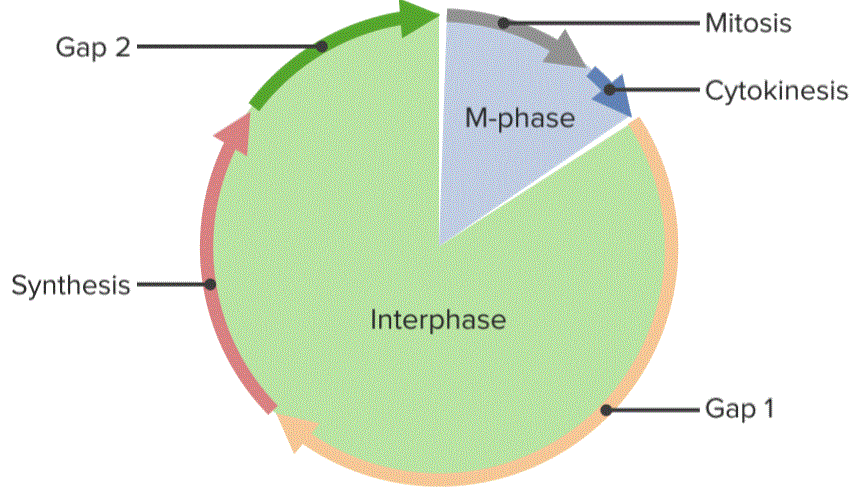
\includegraphics[width=3in]{cellcycle.png}
\end{center}
\caption{Cell cycle, divided into five phases. From \url{https://www.lecturio.com/magazine/the-cell-cycle/}}
\end{figure}

\begin{questions}
\question[1] Which of the following takes place during the portion labeled Gap 1 (G1) phase? Please select all that apply. 
\begin{choices}
\CorrectChoice Growth.
\CorrectChoice Respiration.
\CorrectChoice Doing ``normal'' things that a cell might be specialized/differentiated for.
\CorrectChoice Moving things across the cell membrane. 
\choice Replication of DNA. 
\end{choices}

\question[1] Which of the following takes place during the portion labeled Synthesis (S) phase? Please select all that apply. 
\begin{choices}
\CorrectChoice Growth.
\CorrectChoice Respiration.
\CorrectChoice Doing ``normal'' things that a cell might be specialized/differentiated for.
\CorrectChoice Moving things across the cell membrane. 
\choice Replication of DNA. 
\end{choices}

\question[1] Which of the following takes place during the portion labeled Gap 2 (G2) phase? Please select all that apply. 
\begin{choices}
\CorrectChoice Synthesis of proteins etc that are needed to enable or guide cell division.
\choice Regular ``vanilla'' growth.
\choice Replication of DNA.
\choice Phagocytosis.
\choice Apoptosis.  
\end{choices}

\clearpage
\question[1] Which of the following takes place during the portion labeled M phase? Please select all that apply. 
\begin{choices}
\CorrectChoice Prophase
\CorrectChoice Metaphase
\CorrectChoice Anaphase
\CorrectChoice Telophase
\CorrectChoice Cytokinesis
\end{choices}

\question[1]  What is a ``big'' question you are interested in about cell division (no wrong answers)? 
\begin{solution}[1in]
\end{solution}

\end{questions}
\end{document}